\subsection{Scenario Definition}

The simulation starts in January 2014 and lasts until transition to 100\% SFRs 
is complete. The nuclear installed capacity is constant (100GWe).

\begin{figure}[htpb!]
\begin{center}
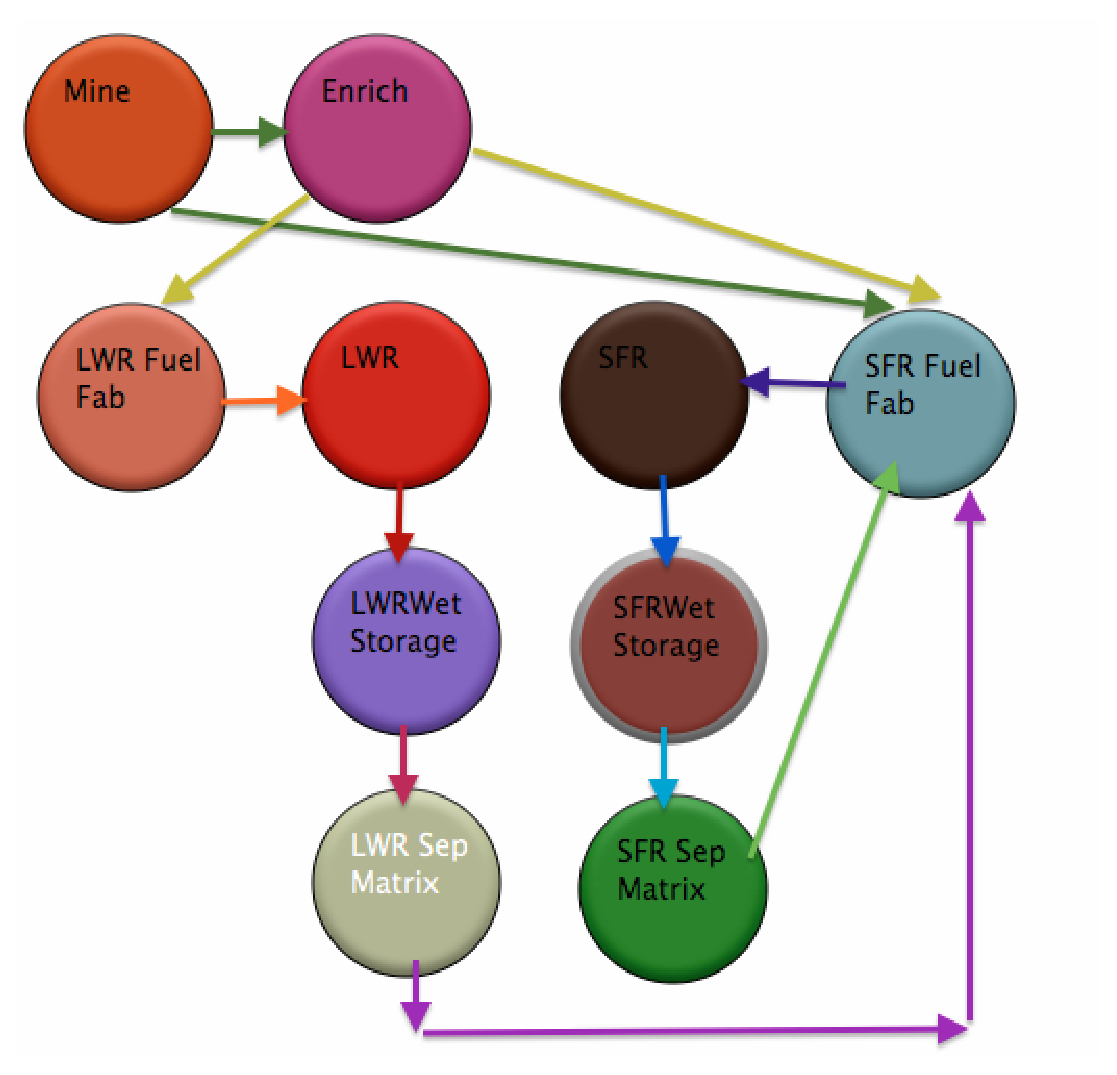
\includegraphics[width=0.45\textwidth]{cycic_img.eps}
\end{center}
\caption{The basic material flow paths for this simulation. This image was 
generated by Cycic, the input controller for Cyclus 
\cite{flannagan_cycic_2013}.}
\label{fig:cycic_img}
\end{figure}

\subsubsection{Deployment Regions and Institutions}

In order to facilitate a deployment profile for the LWR to SFR transition, an 
existing Cycamore model was used. The GrowthRegion model maintains a 
power generation profile specified by the user. It does this by deploying or 
decommissioning reactors when necessary to maintain the specified growth 
profile.  

In this case, a constant 100GWe ``growth'' is maintained in the simulation. 
This region encapsulates all of the facilities in this simulation. 
When sufficient material is available to support a new set of three SFRs, an 
LWR is decommissioned. When power generating capacity is lost due to an LWR 
(1000MWe) decommissioning, the GrowthRegion deploys sufficient SFR capacity 
(three 333.3MWe SFRs) to replace it. 

An entity that decommissions LWRs based on material availability was not 
present in the default models, however. To support this ability, an extension 
model was implemented as a ``Decommissioning Facility.'' That model is 
addressed in Section \ref{sec:decomminst}.

\subsubsection{Commodities}

%\begin{multicols}{1}
\begin{table}[htbp]
\centering
\begin{tabular}{|l|l|l|}
\hline
Commodity  &     Offered By  &    Requested By \\
\hline
Natural  U & Mine & Enrichment \\ 
LEU & Enrichment & LWRFuelFab \\ 
Depleted U & Enrichment & SFRFuelFab \\ 
fresh LWR fuel & LWRFuelFab & LWR \\ 
fresh SFR fuel & SFRFuelFab & SFR \\ 
LWR UNF & LWR & LWRWetStorage \\ 
SFR UNF & SFR & SFRWetStorage \\ 
cool LWR UNF & LWRWetStorage & LWRSeparation \\ 
cool SFR UNF & SFRWetStorage & SFRSeparation \\ 
separated LWR U & LWRSeparation & SFRFuelFab \\ 
separated LWR TRU & LWRSeparation & SFRFuelFab \\ 
separated SFR U & SFRSeparation & SFRFuelFab \\ 
separated SFR TRU & SFRSeparation & SFRFuelFab \\ 
\hline
\end{tabular}
\caption{Commodity movement in the transition simulation}
\label{tab:commods}
\end{table}
%\end{multicols}

Note that the exact compositions of U and TRU were not given. These will be
approximated by representative isotopes in the Cyclus definition.


\subsubsection{Facility Implementations}

\onecolumn
\begin{table}
\centering
\begin{tabular}{|l|l|r|}
\hline
\textbf{Facility Type} &\textbf{Model} & \textbf{Parameters}\\
\hline
Mine & SourceFacility & Capacity = Unlimited\\
Enrichment & EnrichmentFacility & Natural U enrichment = 0.711 wt\% \\
& & Depleted U enrichment =  0.25 wt\% \\
& & ''Enrichment Time'' for LWR fuel = 1 year\\
LWRFuelFab & StreamBlender & Fabrication time = 1 year\\
& & Fissionable material source = 4.3\% LEU\\
SFRFuelFab & StreamBlender  & Fabrication time = 1 year\\
& & fissile material = rep sfr tru, rep lwr tru \\
& & fertile material = rep sfr u, rep lwr u, dep u, nat u \\
LWR & BatchReactor & 1000 MWe per reactor \\
& & 0.90 Capacity Factor \\
& & 3 batches per core \\ 
& & Deployment : initial 2014 deployment only (100 LWRs) \\
& & Decommissioning : decommission 1 LWR per 3 SFRs built \\
& & Burnup = 50 MWd/kgIHM \\
& & Cycle length = 1.5 calendar years \\
& & Licensing time = 2 years \\
& & Construction time = 4 years \\
& & goal recipe \\
SFR & BatchReactor & 333.3 MWe per reactor (1000/3) \\
& & 0.90 Capacity Factor \\
& & Deployment : deploy 3 when 83515 tons LWR UNF available \\ 
& & Decomissioning (after 60 years) \\
& & 3.3 batches per core? \\ 
& & Burnup = 73 MWd/kgIHM \\
& & Cycle length = 1.3 calendar years \\
& & Licensing time = 2 years \\
& & Construction time = 4 years \\
LWRWetStorage & CommodConverter & process time = 4 years\\
SFRWetStorage & CommodConverter & process time = 1 year \\
LWRWetSeparation & SeparationMatrix & Start Date : when needed\\
& & Unlimited Capacity\\
& & No reprocessing losses\\
SFRWetSeparation & SeparationMatrix & Start Date : when needed\\
& & Unlimited Capacity\\
& & No reprocessing losses\\
\hline
\end{tabular}
\caption{Facilities and their Implementations in the simulation.}
\label{tab:facimpl}
\end{table}
\twocolumn


\subsubsection{Desired Outputs}

The desired outputs of this simulation include deployment metrics such as the 
year during which the transition becomes complete and capacity profiles over 
time. These profiles should demonstrate that there were no potential generating 
shortages. Additionally, material metrics such as separated surplus PU or TRU 
profiles, LWR used fuel reprocessing rate (t/yr), SFR used fuel reprocessing 
rate (t/yr),  LWR used fuel mass in storage (t), and SFR used fuel mass in 
storage (t).
